% Graduation thesis — follows Sample_Latex_Thesis2026.tex (Department of Mathematics, IU).
% Build: tectonic Thesis.tex (with DSR) and tectonic Thesis_noDSR.tex (without the DSR subsection).
\documentclass[12pt,a4paper,oneside]{book}
\usepackage{amssymb,amsthm,amsmath,amsfonts}
\renewcommand{\qedsymbol}{}
\usepackage{graphicx}
\usepackage[left= 3cm,right= 3cm,top=3cm,bottom=3cm]{geometry}
\usepackage{subcaption}
\usepackage{bm}
\usepackage{makecell}
\usepackage{longtable}
\usepackage{setspace}
\usepackage{enumerate}
\usepackage{color}
\usepackage{multicol}
\usepackage{multirow}
\usepackage{indentfirst}
\usepackage{float}
\usepackage{framed}
\usepackage{hyperref}
\usepackage{fancyhdr}
\usepackage[utf8]{inputenc}
\usepackage{booktabs}
\usepackage{tabularx}
\usepackage{algorithm}
\usepackage{algorithmic}
\theoremstyle{definition}
\newtheorem{definition}{Definition}[section]
\newtheorem{remark}{Remark}[section]
\pagestyle{fancy}
\renewcommand{\headrulewidth}{0.1pt}
\fancyhf{}
\lhead{\nouppercase{\leftmark}}
\cfoot{\thepage}
\linespread{1.5}
\setlength{\emergencystretch}{2em}

\usepackage{tikz}
\usetikzlibrary{calc,positioning,arrows.meta}
\usepackage{qrcode}

\newcolumntype{L}{>{\raggedright\arraybackslash}X}
\newcommand{\code}[1]{\texttt{#1}}

% Thesis_noDSR.tex defines \nodsr before \input-ing this file.
\newif\ifdsr
\ifdefined\nodsr \dsrfalse \else \dsrtrue \fi

\newcommand{\thesistitle}{LLM-GUIDED, DIMENSION-CONSTRAINED MONTE CARLO TREE SEARCH FOR FORMULAIC ALPHA DISCOVERY IN VN30F INDEX FUTURES}
\newcommand{\studentname}{NGUYEN TRUNG ANH}
\newcommand{\studentid}{MAMAIU22123}
\newcommand{\supervisor}{ASSOC. PROF. TRAN VU KHANH, Ph.D}
\newcommand{\thesisdate}{November 2026}

\begin{document}
	\begin{titlepage}
		\begin{center}
			\bf{VIETNAM NATIONAL UNIVERSITY – HO CHI MINH CITY}\\
			\bf{INTERNATIONAL UNIVERSITY}\\
			\bf{DEPARTMENT OF MATHEMATICS}\\
			\hfill
			\begin{center}
				
\includegraphics[scale=0.6]{logo.png}
			\end{center}
			\vspace*{1 cm}

			\bf  {GRADUATION THESIS}
			\vspace*{1 cm}

			{\large\bf \thesistitle}\\
			\smallskip
			\bf {Submitted in partial fulfillment of the requirements for the degree of}\\
			\bf {BACHELOR OF SCIENCE}\\
			\bf {IN APPLIED MATHEMATICS}\\
			\bf {SPECIALIZATION IN FINANCIAL ENGINEERING }\\
			\bf {AND RISK MANAGEMENT}\\

			\vspace*{1 cm}
		\end{center}
		\begin{tabular}{ll}
			\bf Student's Name:  &\bf \studentname \\
			\bf Student's ID:   &\bf \studentid \\
			\bf Thesis Supervisor:&\bf \supervisor\\
		\end{tabular}

		\vspace*{1cm}
		\begin{center}
			{\bf Ho Chi Minh City, Vietnam}\\
			{\bf \thesisdate}\\
		\end{center}

		\newpage
		\thispagestyle{empty}
		\begin{center}
			\large\textbf{\thesistitle} \\
			\normalsize{By}\\
			\large{\studentname}\\
			\vskip10mm
			\normalsize{Submitted to DEPARTMENT OF MATHEMATICS,\\INTERNATIONAL UNIVERSITY, HO CHI MINH CITY\\ in partial fulfillment of requirements for the degree of\\
				BACHELOR OF SCIENCE \\
				IN APPLIED MATHEMATICS \\
				SPECIALIZATION IN FINANCIAL ENGINEERING  \\
				AND RISK MANAGEMENT}\\
			\thesisdate
			\vskip30mm
		\end{center}
        Signature of Student:
        \rule[0em]{26.7em}{0.5pt}
            \begin{flushright}\studentname \end{flushright}
		\vskip10mm
		Certified by: \rule[0em]{30em}{0.5pt}
		\begin{flushright} \supervisor\\ Thesis Supervisor
		\end{flushright}
		\vskip10mm
		Approved by:
        \rule[0em]{30em}{0.5pt}
        \begin{flushright} ASSOC. PROF. MAI DUC THANH, Ph.D\\ ACTING HEAD OF DEPARTMENT OF MATHEMATICS
        \end{flushright}
	\end{titlepage}

	\newpage
	\thispagestyle{plain}
	\addcontentsline{toc}{chapter}{\numberline{}ABSTRACT}
	\begin{center}
		\large\textbf{\thesistitle} \\
		\normalsize{By}\\
		\large{\studentname}\\
		\vspace*{0.5cm}
	\large\textbf{ABSTRACT}\\
	\end{center}
	\vskip2mm
Automated alpha-mining systems are usually judged by the strategies they produce, yet the best of many tried formulas looks good even when a market contains no exploitable structure. This thesis evaluates the discovery \emph{procedure} of an LLM-guided Monte Carlo Tree Search (MCTS) system for VN30F1M index futures, in which a small local language model proposes formula skeletons, revises them once after seeing training results, and MCTS completes them inside a dimension-typed grammar. The configuration was frozen before the real data were used. A walk-forward run over seven windows yields 877 out-of-sample days (July 2022 to December 2025); the system is compared with MCTS without the LLM, random search, the LLM without search, buy-and-hold and time-series momentum, with 19 placebo runs on permuted returns and a planted-signal benchmark as controls. The full system reached an out-of-sample Sharpe ratio of 0.68, matched or exceeded by 2 of 19 placebo runs ($p = 0.15$); its five-seed mean (0.44) was indistinguishable from MCTS without the LLM (0.40) and random search (0.46). On planted signals the LLM did not raise the recovery rate (Holm-adjusted $p \ge 0.94$), and only one of four planted formulas was detected, at an information coefficient of 0.1. The result is negative: no evidence that the system discovers more than chance on VN30F1M, nor that LLM guidance improves the search. The contribution is the evaluation protocol that makes such a statement possible for a single instrument.
\vskip10mm
\textbf{Keywords:} Formulaic alpha, Monte Carlo Tree Search, large language models, data snooping, walk-forward evaluation, permutation test, planted signal, VN30F.

\newpage
\clearpage
\chapter*{ACKNOWLEDGEMENT}
\addcontentsline{toc}{chapter}{ACKNOWLEDGEMENT}

I would like to thank my supervisor, Assoc. Prof. Tran Vu Khanh, for his guidance and feedback throughout this work, and the Department of Mathematics, International University, for the education and support that made it possible.

\chapter*{DECLARATION ON THE USE OF AI TOOLS}
\addcontentsline{toc}{chapter}{DECLARATION ON THE USE OF AI TOOLS}

An AI coding assistant (Claude, Anthropic) was used during this project to write and test parts of the source code, to review the methodology, and to draft parts of this text. The research questions, the design decisions recorded in the project's decision log, and the interpretation of the results are the author's; every number reported here was produced by the code in the public repository and checked against its result files. The local language model studied in the thesis (\code{qwen3.5:4b}) is the object of the experiments, not a writing aid.

	\newpage
	\clearpage

	\mainmatter
	\tableofcontents
	\newpage
	\clearpage

\listoffigures
\newpage
\clearpage

\listoftables
\newpage
\clearpage

\chapter*{List of Abbreviations}
\addcontentsline{toc}{chapter}{List of Abbreviations}
\begin{description}
    \item[CI] Confidence Interval
\ifdsr
    \item[DSR] Deflated Sharpe Ratio
\fi
    \item[HMM] Hidden Markov Model
    \item[IC] Information Coefficient (Spearman correlation between a signal and the next-bar return)
    \item[LLM] Large Language Model
    \item[MCTS] Monte Carlo Tree Search
    \item[OHLCV] Open, High, Low, Close, Volume
    \item[OOS] Out-of-Sample
\ifdsr
    \item[PSR] Probabilistic Sharpe Ratio
\fi
    \item[RQ] Research Question
    \item[SPA] Superior Predictive Ability (test)
    \item[TSMOM] Time-Series Momentum
    \item[UCT] Upper Confidence bounds applied to Trees
    \item[VN30F1M] VN30 index futures, front-month contract
\end{description}

\clearpage

%══════════════════════════════════════════════════════════════════════════════
\chapter{INTRODUCTION}
\label{ch1}

\section{Motivation and Background}

Quantitative trading signals, or \emph{alphas}, are often written as explicit formulas over price and volume, such as the 101 alphas published by Kakushadze \cite{kakushadze2016}. Because the space of such formulas is combinatorial, a growing body of work searches it automatically, first with genetic programming \cite{koza1992} and reinforcement learning \cite{yu2023,xu2024}, and more recently with large language models (LLMs), alone \cite{wang2023,tang2025} or combined with Monte Carlo Tree Search (MCTS) \cite{ren2024,shi2026}. These systems are typically evaluated by the alphas they return: a training period is searched, the best formulas are combined, and the combination is scored on a later test period.

That evaluation answers a narrower question than it appears to. A search that tries tens of thousands of formulas and keeps the best will find formulas that look profitable on the searched data even when nothing is there to find \cite{white2000,harvey2015,harvey2016}. Whether the \emph{procedure} finds real structure can only be judged against what the same procedure produces when no structure exists, and against what it recovers when a known structure is planted. For a single instrument the problem is sharper still: with one futures contract, evidence accumulates only over time, and a few years of out-of-sample returns can separate only large edges from luck \cite{lo2002}.

This thesis studies such a system for VN30F1M, the front-month VN30 index futures contract and the most liquid derivative traded in Vietnam. A local LLM proposes the structure of a strategy (a \emph{blueprint}), MCTS completes the formula inside a grammar where every node carries a physical dimension, and each candidate is scored by a backtest that models the fees, margin and margin calls of the Vietnamese derivatives market. After a first search phase, the LLM sees the best formulas found so far and writes new blueprints, which a second phase completes.

\section{Problem Statement}

The question addressed is not whether a particular alpha is good, but whether the discovery procedure, applied to VN30F1M as a researcher would apply it in real time, produces trading strategies better than chance, and whether the LLM contributes to that. Answering it requires (i) out-of-sample evidence collected as if the procedure had been run at successive points in the past, (ii) a null distribution of the procedure's own output on data without predictable structure, (iii) a check that the procedure can find a structure of known strength when one is present, and (iv) comparisons with alternative procedures under the same budget. It also requires that every choice be fixed before the real out-of-sample data are used, since any adjustment after seeing them would reintroduce the selection bias the protocol is meant to remove.

\section{Research Questions}
\label{sec:rqs}

\begin{enumerate}
  \item[\textbf{RQ1.}] \textbf{Role of the LLM.} Under the same limit on formula size and the same evaluation budget, does LLM guidance lead MCTS to a true signal more often than MCTS without the LLM, or does it block the way? The primary measurement is the planted-signal benchmark (Section~\ref{sec:planted}); the out-of-sample Sharpe ratios of all configurations in the real walk-forward run are reported descriptively.
  \item[\textbf{RQ2.}] \textbf{Evidence of discovery.} Is the out-of-sample performance of the full system higher than what the same procedure achieves on placebo data without predictable structure, and which planted signals can the procedure recover?
\end{enumerate}

These questions differ from those of the proposal; Section~\ref{sec:deviations} lists the changes and the reasons for them.

\section{Contributions}

\begin{enumerate}
  \item An evaluation protocol for automated alpha discovery on a single instrument, combining a frozen pre-registered configuration, walk-forward evaluation of alpha sets, equal-budget comparison with ablated and random procedures, a placebo test that repeats the whole procedure, and a planted-signal benchmark that measures the detection threshold.
  \item A negative result for VN30F1M: under this protocol, the LLM-guided system shows no evidence of discovering more than chance, and the LLM does not measurably improve the search compared with MCTS alone or with random sampling of the same grammar.
  \item An open-source implementation, including all result files and the commands that produce every number in this thesis.
\end{enumerate}

\section{Scope}

The study covers one instrument, VN30F1M, using 60-minute OHLCV bars from the broker DNSE between 13 August 2018 and 31 December 2025. Signals are directional (long, short or flat). The LLM is a small model (\code{qwen3.5:4b}, about four billion parameters) run locally through Ollama; no cloud model is used. Cross-sectional stock portfolios, live trading and other bar frequencies are out of scope.

The rest of the thesis is organised as follows. Chapter~\ref{ch2} reviews the literature. Chapter~\ref{ch3} describes the data, the discovery system, the configurations and the evaluation protocol. Chapter~\ref{ch4} reports the results. Chapter~\ref{ch5} discusses them and their limitations, and Chapter~\ref{ch6} concludes.

%══════════════════════════════════════════════════════════════════════════════
\chapter{LITERATURE REVIEW}
\label{ch2}

\section{Formulaic Alphas and Automated Search}

Kakushadze \cite{kakushadze2016} published 101 formulaic alphas used in practice, built from ranks, delays, differences, correlations and rolling extrema of price and volume. The space of such formulas has been searched with genetic programming \cite{koza1992}, with reinforcement learning that generates sets of alphas working well in combination \cite{yu2023}, and with tree search \cite{xu2024,ren2024}, building on the UCT rule of MCTS \cite{kocsis2006,browne2012}. RiskMiner \cite{ren2024} replaces the average reward of UCT with a risk-seeking criterion that favours the best outcome below a node, which suits a search whose goal is a few excellent formulas rather than a good average.

\section{LLMs in Alpha Mining}

Alpha-GPT \cite{wang2023} turns research ideas stated by a human into alpha expressions. AlphaAgent \cite{tang2025} lets an LLM agent propose hypotheses and formulas, penalising formulas whose syntax tree duplicates existing alphas. The framework of Shi et al. \cite{shi2026} uses an LLM inside MCTS to generate and refine formulas at each node from backtest feedback, in the spirit of self-refinement \cite{madaan2023}. Beyond alpha mining, LLMs have been used to read news and predict returns \cite{lopezlira2023}, a setting in which Glasserman and Lin \cite{glasserman2023} showed that the model's training data can leak future information, and that hiding company names reduces this look-ahead bias.

\section{How Alpha-Mining Systems Are Evaluated}

The studies above share an evaluation protocol. The system is run on a training period, the alphas it produces are combined, and the combination is evaluated on a later test period: 2011--2020 versus 2021--2024 in \cite{shi2026}, 2010--2019 versus 2021--2022 in \cite{ren2024}, 2009--2018 versus 2021--2023 in \cite{xu2024}. Performance is measured by the information coefficient, complemented in \cite{shi2026,ren2024} by trading simulations, and compared against other mining methods. All of these studies are cross-sectional: each test day contributes hundreds of stocks, so even a small information coefficient can be estimated precisely.

Table~\ref{tab:checklist} summarises how four LLM-based studies handle the threats to validity that this thesis addresses. None of them compares the system with a version without the LLM under the same budget, with random search, with the same procedure on placebo data, or with a planted signal of known strength. The leakage test of Shi et al. \cite{shi2026}, which asks LLMs to write formulas directly and finds them no better than random, is the closest to an ablation, and it motivates the ``LLM only'' configuration of this thesis.

\begin{table}[H]
\centering
\caption{Evaluation practice in LLM-based alpha mining (\checkmark{} present, $\sim$ partial or unclear, -- absent)}
\label{tab:checklist}
\setstretch{1.1}
\small
\begin{tabularx}{\textwidth}{Lcccc}
\toprule
\textbf{Item} & \textbf{\cite{wang2023}} & \textbf{\cite{tang2025}} & \textbf{\cite{shi2026}} & \textbf{This thesis} \\
\midrule
Test period separated in time, not used for selection & -- & $\sim$ & $\sim$ & \checkmark \\
Transaction costs & -- & $\sim$ & \checkmark & \checkmark \\
Several runs / significance test & -- & $\sim$ & -- & \checkmark \\
Same budget without LLM; random search & -- & -- & -- & \checkmark \\
Leakage through LLM weights & $\sim$ & -- & \checkmark & $\sim$ \\
Placebo test of the whole procedure & -- & -- & -- & \checkmark \\
Planted-signal benchmark & -- & -- & -- & \checkmark \\
\bottomrule
\end{tabularx}
\end{table}

\section{Data Snooping and Statistical Significance}

When a model is selected from a search, its performance must be compared with the distribution of the \emph{best} of all tried models: the Reality Check of White \cite{white2000} and the SPA test of Hansen \cite{hansen2005}. Aronson \cite{aronson2006} applied such tests and Monte Carlo permutations to technical trading rules, and Masters \cite{masters2020} extends permutation tests to entire trading-system development procedures: the procedure is rerun on many permuted datasets, and the real result is ranked among the permuted ones. Backtested Sharpe ratios can be haircut for the number of trials \cite{harvey2015,harvey2016} or deflated \cite{bailey2014}, and the probability of backtest overfitting can be estimated \cite{bailey2017}. Lo \cite{lo2002} gives the sampling distribution of the Sharpe ratio, which fixes how much data is needed to detect an edge, and Ledoit and Wolf \cite{ledoit2008} discuss tests of the difference between two Sharpe ratios. Synthetic data with known properties let one check whether a method recovers what is there \cite{lopezdeprado2018,arian2024}.

\section{Research Gap}

\begin{enumerate}
  \item Evaluation protocols for alpha-mining systems were developed for cross-sectional equities. For a single instrument the same protocol has far less statistical power, and the studies reviewed do not address how to compensate.
  \item Published LLM-based systems are compared with each other, but not with what the same procedure finds when no signal exists, not with the same search without the LLM, and not on their ability to recover a known signal.
  \item No study evaluates an LLM-guided search for directional signals on Vietnamese index futures.
\end{enumerate}

%══════════════════════════════════════════════════════════════════════════════
\chapter{METHODOLOGY}
\label{ch3}

\section{Data and Market}
\label{sec:data}

VN30F1M is the front-month futures contract on the VN30 index, traded on the Hanoi Stock Exchange. The data are 60-minute OHLCV bars from the broker DNSE, 13 August 2018 to 31 December 2025, of the continuous front-month series. The backtest uses the contract specifications in Table~\ref{tab:contract}. Files at finer frequencies (1 to 30 minutes) miss 126 trading sessions between March 2023 and March 2024 compared with the 60-minute file; they are not used.

\begin{table}[H]
\centering
\caption{Contract and backtest parameters}
\label{tab:contract}
\setstretch{1.1}
\begin{tabular}{ll}
\toprule
Multiplier & 100,000 VND per index point \\
Fee & 6,000 VND per contract per side \\
Initial margin / maintenance margin & 28.5\% / 20\% \\
Initial capital & 1 billion VND \\
Execution & a signal at bar $t$ fills at bar $t+1$ \\
Margin call & position flattened, equity frozen \\
\bottomrule
\end{tabular}
\end{table}

The backtest receives a series of target positions. The number of contracts is fixed from the initial capital and the first price, so that returns are comparable across strategies, and a daily return is the change in end-of-day equity divided by the initial capital. All annualisation goes through one function: the Sharpe ratio is the mean over the standard deviation of daily returns, multiplied by $\sqrt{252}$.

\section{The Discovery System}
\label{sec:system}

\subsection{Grammar with Dimensions}

A formula is a tree whose leaves are the fields \code{open}, \code{high}, \code{low}, \code{close}, \code{volume} or constants, and whose internal nodes are drawn from 19 operators: nine rolling time-series operators (\code{ts\_mean}, \code{ts\_sum}, \code{ts\_max}, \code{ts\_min}, \code{ts\_rank}, \code{ts\_zscore}, \code{ts\_argmax}, \code{ts\_argmin}, \code{ts\_corr}), six logical operators (\code{greater\_than}, \code{less\_than}, \code{equal}, \code{and\_}, \code{or\_}, \code{not\_}) and four arithmetic operators (\code{add}, \code{sub}, \code{mult}, \code{div}). Every node carries a dimension: price, volume, ratio or boolean. Rolling means, sums and extrema keep the dimension of their input; ranks, z-scores, arg-extrema and correlations return a ratio; \code{add} and \code{sub} require equal dimensions; \code{mult} requires one ratio factor; comparisons require equal dimensions and return a boolean. Formulas such as price plus volume are therefore never generated. The dimension of every open slot is inferred in both directions through the tree, so that each slot is offered only fields and operators that can still complete a valid formula within the depth limit of four. Each rolling operator has its own window, chosen by the search from $\{2, 3, 5, 10\}$ bars.

\subsection{Position Templates}

The root dimension of a formula decides how it becomes a position in $\{-w, 0, +w\}$ with $w = 0.2$:
\begin{itemize}
  \item \textbf{NORMALIZED} (price or volume roots): the rolling z-score of the formula over a window in $\{2,3,5,7,10\}$ is compared with $\pm\theta$, $\theta \in \{0.5, 1.0, 1.5, 2.0, 2.5\}$;
  \item \textbf{RATIO}: the formula is compared with an upper threshold in $\{60,\dots,80\}$ and a lower threshold in $\{20,\dots,40\}$;
  \item \textbf{BOOLEAN}: long when true, short when false.
\end{itemize}
Each formula is tried in both directions and the better one is kept.

\subsection{Reward}

A candidate is scored on the training segment by
\begin{equation}
R = 0.6\, S_{\mathrm{sharpe}} + 0.4\, S_{\mathrm{IC}}, \qquad
S_{\mathrm{sharpe}} = \mathrm{clip}\!\left(\frac{\mathrm{SR}}{3}, 0, 1\right), \qquad
S_{\mathrm{IC}} = \min\!\left(1, \frac{|\mathrm{IC}|}{0.15}\right),
\label{eq:reward}
\end{equation}
where SR is the annualised Sharpe ratio of the backtest after costs and IC is the Spearman correlation between the signal and the next-bar return (for NORMALIZED formulas, the z-scored signal that is actually traded). $S_{\mathrm{sharpe}} = 0$ when the candidate makes fewer than 15 trades. Formulas whose evaluation fails, typically because a rolling operator receives an expression of constants only, score $-10$. This reward was fixed before any thesis run.

\subsection{Monte Carlo Tree Search}

MCTS completes the open slots of a blueprint one decision at a time: an operator, field or constant for a slot, a window for a rolling operator, or a template parameter. Selection uses UCT with the \emph{maximum} reward below a node in place of the mean, with exploration constant $c = 1.414$, following the risk-seeking idea of \cite{ren2024}. Evaluated formulas are cached. All randomness goes through one seeded generator, so that a seed, a dataset and a blueprint set determine the leaderboard exactly. Early stopping is disabled in the configurations compared, so each spends its full budget; the search phases of the full system run interleaved in blocks of 500 iterations per blueprint.

\subsection{Blueprints from the LLM}

The LLM is \code{qwen3.5:4b}, run locally through Ollama with temperature 0.3, a context of 32,768 tokens and its reasoning (``thinking'') mode on; each request is limited to 16,384 generated tokens and retried up to twice with the next seed if cut off. The prompt describes the operators, the dimension rules and four structural ``shapes'' that may not be copied; it does not name the market or the instrument, to reduce leakage of remembered price history \cite{glasserman2023}. The LLM returns blueprints such as \code{sub(ts\_max(?), ts\_min(?))}, in which every \code{?} is an open slot for MCTS. A blueprint is accepted only if it compiles, passes the dimension check, has at least one slot, can be completed within the depth limit, and is not structurally identical to a prompt example or to another accepted blueprint. Rejected blueprints are returned to the LLM once, with the reasons, for correction.

The initial set of 20 blueprints was generated once (seed 2026) and frozen; it is listed in Appendix~\ref{app:blueprints}. It uses 16 of the 19 operators and admits about $2.2 \times 10^{14}$ completions, against about $1.9 \times 10^{41}$ formulas in the whole grammar at the same depth.

\subsection{The Feedback Round}
\label{sec:feedback}

Each run of the full system spends 100,000 evaluations in two phases (Figure~\ref{fig:arch}):
\begin{enumerate}
  \item \textbf{Phase A.} The 20 frozen blueprints, 2,500 MCTS iterations each (50,000 evaluations), on the training segment.
  \item \textbf{Feedback.} The 10 best distinct formulas by training reward are shown to the LLM with their reward and training IC. Windows are removed from the formulas, and formulas that differ only in windows are merged. Validation and evaluation data are never shown. The LLM writes 10 new blueprints in one request, under the same acceptance rules and not duplicating the initial set.
  \item \textbf{Phase B.} The new blueprints, 5,000 iterations each (50,000 evaluations). If the feedback round yields no accepted blueprint, phase B falls back to the initial set.
\end{enumerate}
The Ollama seed is fixed by the run and the MCTS seed, so a rerun produces the same blueprints.

\begin{figure}[H]
\centering
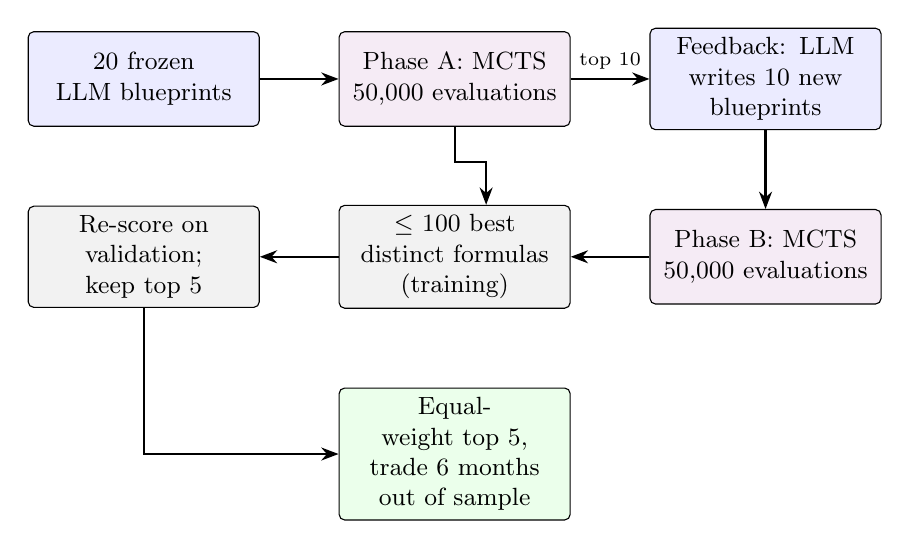
\begin{tikzpicture}[
  node distance=1.0cm and 1.0cm,
  box/.style={draw, rounded corners=2pt, align=center, font=\small\setstretch{1.0}, minimum height=1.2cm, text width=2.7cm, fill=#1},
  box/.default={white},
  arr/.style={-{Stealth[length=2.2mm]}, thick},
  lbl/.style={font=\scriptsize, align=center, fill=white, inner sep=1pt}]
  \node[box=blue!8] (bp) {20 frozen\\LLM blueprints};
  \node[box=violet!8, right=of bp] (a) {Phase A: MCTS\\50,000 evaluations};
  \node[box=blue!8, right=of a] (fb) {Feedback: LLM\\writes 10 new\\blueprints};
  \node[box=violet!8, below=of fb] (b) {Phase B: MCTS\\50,000 evaluations};
  \node[box=gray!10, left=of b] (rank) {$\le$ 100 best\\distinct formulas\\(training)};
  \node[box=gray!10, left=of rank] (val) {Re-score on\\validation;\\keep top 5};
  \node[box=green!8, below=of rank] (trade) {Equal-weight top 5,\\trade 6 months\\out of sample};
  \draw[arr] (bp) -- (a);
  \draw[arr] (a) -- node[above, lbl, yshift=2pt]{top 10} (fb);
  \draw[arr] (fb) -- (b);
  \draw[arr] (b) -- (rank);
  \draw[arr] (a.south) -- ++(0,-0.45) -| ([xshift=4mm]rank.north);
  \draw[arr] (rank) -- (val);
  \draw[arr] (val.south) |- (trade.west);
\end{tikzpicture}
\caption{One walk-forward window of the full system (LLM + MCTS with feedback)}
\label{fig:arch}
\end{figure}

\subsection{Selection and Combination}

After the search, at most 100 distinct formulas with the best training rewards (each with its best template parameters) are re-scored on a separate validation segment, and the five best by validation reward form the strategy: their target positions are averaged with equal weights and traded on the evaluation segment. Rolling operators are computed on the continuous series, so the evaluation segment starts with a full history.

\section{Configurations Compared}
\label{sec:configs}

All search configurations receive 100,000 evaluations per window and use the same selection and combination step (Table~\ref{tab:configs}).

\begin{table}[H]
\centering
\caption{Configurations compared}
\label{tab:configs}
\setstretch{1.1}
\small
\begin{tabularx}{\textwidth}{lLc}
\toprule
\textbf{Configuration} & \textbf{Description} & \textbf{Seeds} \\
\midrule
LLM + MCTS & Full system with one feedback round (Section~\ref{sec:feedback}) & 1--5 \\
MCTS only & MCTS from a single open slot under each template (NORMALIZED, RATIO, BOOLEAN), budget split equally; no LLM & 1--5 \\
Random search & 100,000 dimension-valid formulas sampled by size, ramped half-and-half over depths 1--4 \cite{koza1992}; windows and template parameters drawn uniformly; duplicates removed & 1--5 \\
LLM only & The LLM writes 100 complete formulas once (no slots, no data), frozen; each window scores all of them on the template-parameter grid (about 2,500 evaluations) & 1 \\
Buy-and-hold & Always long, same position size, fees and margin & 1 \\
TSMOM & Sign of the past return over $L$ bars \cite{moskowitz2012}, $L \in \{$1 session, 1 week, 1 month$\}$ chosen by validation Sharpe & 1 \\
\bottomrule
\end{tabularx}
\end{table}

The LLM-only configuration is deterministic given its frozen formula set, and the two references have no randomness, so they run with one seed. The LLM-only formula set was generated with 27 requests in about one hour; all 100 formulas were accepted.

\section{Walk-Forward Evaluation}
\label{sec:wf}

The procedure is run as if a researcher had applied it at seven successive dates, each time seeing only the past (Figure~\ref{fig:wf}). The training segment expands from 13 August 2018; the 12 months before each evaluation segment form the validation segment; evaluation segments of six months roll forward by six months from July 2022 to December 2025. The training segments contain 3,583 bars (window 1) to 7,319 bars (window 7); validation segments 1,239 to 1,249 bars; evaluation segments 595 to 650 bars. The seven evaluation segments are concatenated into one series of 877 daily out-of-sample returns, whose annualised Sharpe ratio is the primary metric. For the search configurations the five seeds give five series; their daily mean is reported as a descriptive summary.

\begin{figure}[H]
\centering
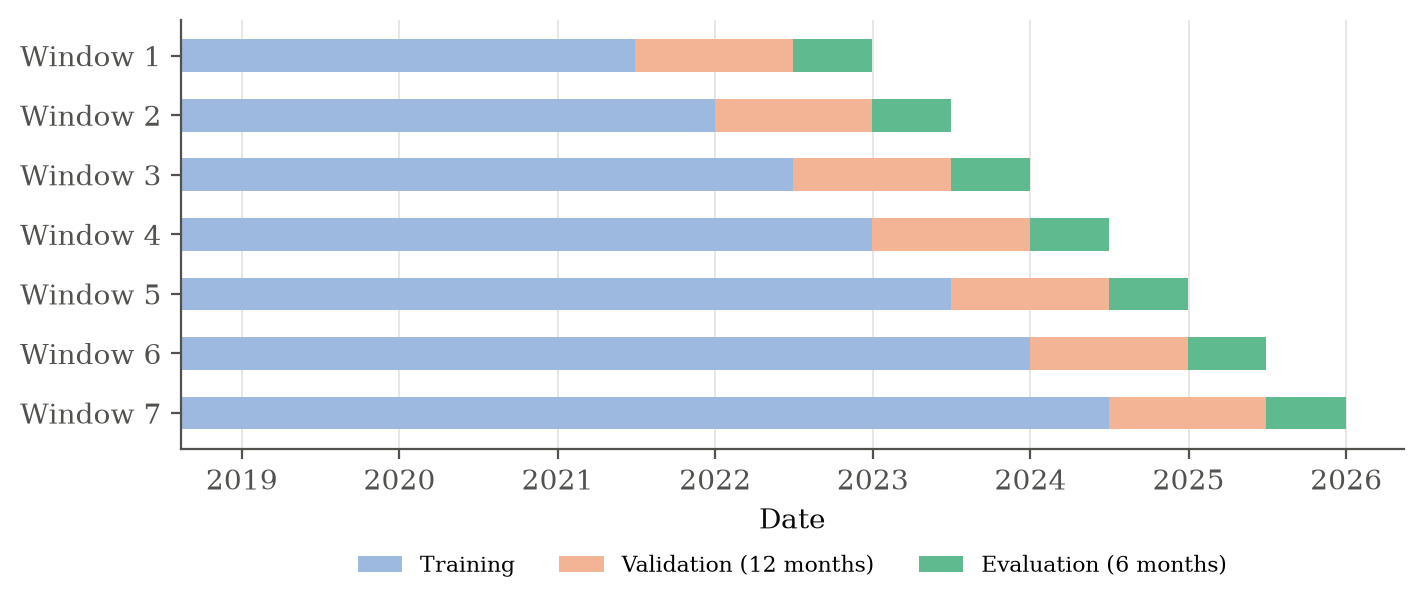
\includegraphics[width=0.9\textwidth]{figures/wf_windows.png}
\caption{Walk-forward windows: expanding training segment, 12-month validation, 6-month evaluation}
\label{fig:wf}
\end{figure}

The data allow only coarse comparisons. The standard error of an annualised Sharpe ratio over 3.5 years is about $1/\sqrt{3.5} \approx 0.54$ \cite{lo2002}. For the difference of two Sharpe ratios estimated on the same 877 days, the variance of the difference depends on the correlation $\rho$ of the two daily return series \cite{ledoit2008}; with $\rho = 0.7$, a one-sided test at the 5\% level detects a difference of 0.68 with power 50\% and of 1.03 with power 80\%. These numbers were computed before the real run and set the expectations for RQ1: the walk-forward comparison is descriptive.

\section{Placebo Test (RQ2, Negative Control)}
\label{sec:placebo}

To learn what the procedure finds when there is nothing to find, the full walk-forward run of LLM + MCTS is repeated on $K = 19$ placebo datasets. In each placebo set and each window, bar returns are permuted separately within the training, validation and evaluation segments, each bar carrying its own volume and intrabar shape, and prices are rebuilt from the permuted returns; the permutation seed is a fixed function of the set and the window. Permutation destroys any dependence of the next return on the past while keeping the marginal distribution of returns, so every placebo set is a market in which, by construction, no formula has an edge. Because each placebo run repeats the entire procedure, including the LLM feedback round, the selection on validation and the combination of five formulas, the placebo distribution contains all the selection bias of the real run \cite{masters2020}.

The p-value compares the real run with MCTS seed 1, the seed used by every placebo set:
\begin{equation}
p = \frac{1 + \#\{k : \mathrm{SR}_k^{\mathrm{placebo}} \ge \mathrm{SR}^{\mathrm{real}}\}}{K + 1},
\label{eq:pvalue}
\end{equation}
whose smallest attainable value with $K = 19$ is 0.05. The five-seed mean series is not used for the p-value, because averaging five portfolios lowers volatility and would favour the real run against single-seed placebo runs.

\section{Planted-Signal Benchmark (RQ1, RQ2, Positive Control)}
\label{sec:planted}

A known formula $A$ is planted in placebo returns with a controlled strength. Starting from permuted returns $\varepsilon$, returns are generated bar by bar:
\begin{equation}
r_{t+1} = \varepsilon_{t+1} + \beta\, \sigma_\varepsilon\, s_t, \qquad s_t = \mathrm{ts\_zscore}(A, 10)_t,
\end{equation}
where $s_t$ is computed on the prices rebuilt up to bar $t$. One $\beta \ge 0$ per strength is found by bisection so that the mean Spearman IC between $s_t$ and $r_{t+1}$ over 20 calibration permutations equals the target IC of 0, 0.05 or 0.1. IC 0 is a pure placebo and measures false discoveries.

Four formulas were fixed before the blueprint set was generated, so that the choice could not follow the blueprints:
\begin{itemize}
  \item A1 \code{ts\_corr(close, volume, 10)} and A2 \code{ts\_mean(close - open, 10)}: two classical signals (price--volume correlation and intraday momentum);
  \item A3 \code{ts\_argmin(volume, 10)} and A4 \code{ts\_argmax(ts\_zscore(volume, 10), 5)}: two unusual signals drawn at random from the grammar with one and two operators.
\end{itemize}
Every $A$ had to be stationary (ADF $p < 10^{-12}$) and rare: fewer than 1\% of 10,000 random formulas may have $|\rho_S| \ge 0.7$ with it (the observed shares were 0.21\%, 0.17\%, 0.30\% and 0.36\%), so that a near recovery cannot happen by accident. A mean-reverting price signal, the first candidate for A1, failed this rule: 6.9\% of random formulas resemble it.

For each configuration (LLM + MCTS, MCTS only, random search), each $A$ and each IC, 10 seeds are run with a budget of 100,000 evaluations, on the segments training 13/08/2018--31/12/2019, validation to 30/06/2020 and evaluation to 31/12/2020; 2025 data are never used in this benchmark. The leaderboard is recorded at 10,000, 25,000, 50,000, 75,000 and 100,000 evaluations, and at each checkpoint the top five are selected on validation as in the real run. A run \emph{recovers $A$ nearly} if one of its top five formulas has $|\rho_S| \ge 0.7$ with $A$ on the search period. In total $3 \times 4 \times 2 \times 10$ runs at IC 0.05 and 0.1 plus $3 \times 10$ at IC 0 give 270 runs; the IC 0 runs are shared by the four $A$, which makes 360 configuration--$A$--IC--seed cells.

\section{Statistical Tests}
\label{sec:tests}

\begin{itemize}
  \item \textbf{RQ1, primary.} LLM + MCTS against MCTS only, at IC 0.1, pooled by type of $A$ (classical A1 + A2, unusual A3 + A4, 20 runs each), at 50,000 evaluations (before feedback) and 100,000 (after): four two-sided Fisher exact tests on near-recovery counts, Holm-adjusted \cite{holm1979}. Two-sided, because the LLM may block the way. All other cells (other ICs, single $A$, other checkpoints, random search) are descriptive.
  \item \textbf{RQ2, detection threshold.} For each $A$, the lowest IC at which the near-recovery rate of LLM + MCTS at 100,000 exceeds that at IC 0 (one-sided Fisher test, 5\%). The rule fixed in advance that, if no $A$ passed at IC 0.1, a level 0.2 would be added.
  \item \textbf{RQ2, placebo.} The p-value \eqref{eq:pvalue}.
  \item \textbf{RQ1, descriptive.} The difference of annualised Sharpe ratios between LLM + MCTS and each other configuration on the 877 daily returns, with a 95\% interval from a paired stationary bootstrap \cite{politis1994} (mean block length 10 days, 10,000 resamples, fixed seed), and the correlation $\rho$ of daily returns.
\ifdsr
  \item \textbf{Supplementary.} The Deflated Sharpe Ratio \cite{bailey2014} of each real out-of-sample series (Section~\ref{sec:dsr}).
\fi
\end{itemize}

\section{Pre-Registration and Freeze}
\label{sec:freeze}

The protocol was designed to be run once on the real data. All tuning of prompts, parameters and code took place on permuted data, on the planted-signal benchmark and on the placebo runs. Before the real walk-forward run, a freeze file recorded the reward and its weights, the window table, the SHA-256 of the blueprint set and of the LLM-only formula set, the template grids, the TSMOM grid, the budget, the LLM, the seeds of every configuration, the git commit of the code and a fingerprint of the data. The run command refuses to start if any of these differ, or if any file of the engine or the workflows has changed since the frozen commit. The real run was started once, on 2 November 2026, and not repeated.

\section{Deviations from the Proposal}
\label{sec:deviations}

\begin{enumerate}
  \item \textbf{Research questions.} The proposal's RQ2 (primitive operators versus technical indicators) was dropped: indicators are themselves compositions of primitive operators, and with a detection threshold near IC 0.1 the comparison would almost surely be inconclusive. The former RQ3 became RQ2.
  \item \textbf{Measurement of RQ1.} The proposal measured RQ1 by out-of-sample Sharpe ratios. With 877 days only differences of about one Sharpe unit are detectable (Section~\ref{sec:wf}), so the primary measurement moved to the planted-signal benchmark, where noise is controlled; the walk-forward comparison is reported descriptively.
  \item \textbf{Feedback round.} In the proposal the LLM generated blueprints once. A one-shot set only measures how much of the space the set covers, and the small model copied the prompt's examples (\code{ts\_zscore} appeared in 16 of the first 20 blueprints). One feedback round was therefore added, the prompt was corrected and the blueprint set regenerated.
  \item \textbf{Windows.} The proposal planned eleven windows with two-year searches from July 2020. A planted-signal run showed that two years of 60-minute bars detect only signals of IC 0.1 or more, so the training segment expands from 2018 instead, at the cost of a shorter out-of-sample period (seven windows, 3.5 years).
  \item \textbf{Planted strengths.} IC levels of 0, 0.05 and 0.1 replace the proposal's examples of 0.01--0.05, which lie below the noise level of the available data; results are reported as a detection threshold.
  \item \textbf{SPA and DSR.} The placebo test repeats the whole procedure and therefore already accounts for every trial inside it; it replaces the SPA test as the primary test of RQ2. \ifdsr The Deflated Sharpe Ratio is reported as a supplement (Section~\ref{sec:dsr}).\else The LLM-only configuration, which has no placebo runs, is reported descriptively.\fi
\end{enumerate}

%══════════════════════════════════════════════════════════════════════════════
\chapter{RESULTS}
\label{ch4}

\section{Planted-Signal Benchmark}
\label{sec:res-planted}

\subsection{RQ1: Primary Tests}

Table~\ref{tab:primary} gives the four primary comparisons. None is significant: the largest difference, 6 of 20 against 2 of 20 for classical signals before feedback, has an unadjusted $p$ of 0.235.

\begin{table}[H]
\centering
\caption{RQ1 primary tests: near recoveries at IC 0.1 (out of 20 runs)}
\label{tab:primary}
\setstretch{1.1}
\small
\begin{tabular}{llcccc}
\toprule
\textbf{Budget} & \textbf{Type of $A$} & \textbf{LLM + MCTS} & \textbf{MCTS only} & \textbf{$p$} & \textbf{$p$ (Holm)} \\
\midrule
50,000 & classical (A1 + A2) & 6 & 2 & 0.235 & 0.940 \\
50,000 & unusual (A3 + A4) & 2 & 0 & 0.487 & 0.974 \\
100,000 & classical & 7 & 3 & 0.273 & 0.940 \\
100,000 & unusual & 0 & 1 & 1.000 & 1.000 \\
\bottomrule
\end{tabular}
\end{table}

\subsection{Recovery by Signal}

Table~\ref{tab:recovery} breaks the 100,000-evaluation results down by $A$ and IC, and Figures~\ref{fig:planted-ic} and \ref{fig:planted-budget} show them graphically. No configuration ever recovered a signal at IC 0, so the near-recovery criterion produced no false discoveries. At IC 0.1, LLM + MCTS recovered A2 in 5 of 10 runs, against 1 for MCTS only and 0 for random search; for the other three signals, random search recovered as often as or more often than the two MCTS configurations.

\begin{table}[H]
\centering
\caption{Near recoveries at 100,000 evaluations (out of 10 runs), IC 0 / 0.05 / 0.1}
\label{tab:recovery}
\setstretch{1.1}
\small
\begin{tabular}{lccc}
\toprule
\textbf{$A$} & \textbf{LLM + MCTS} & \textbf{MCTS only} & \textbf{Random search} \\
\midrule
A1 (price--volume correlation) & 0 / 1 / 2 & 0 / 0 / 2 & 0 / 0 / 4 \\
A2 (intraday momentum) & 0 / 1 / \textbf{5} & 0 / 0 / 1 & 0 / 1 / 0 \\
A3 (unusual, 1 operator) & 0 / 1 / 0 & 0 / 0 / 1 & 0 / 0 / 3 \\
A4 (unusual, 2 operators) & 0 / 0 / 0 & 0 / 1 / 0 & 0 / 0 / 1 \\
\bottomrule
\end{tabular}
\end{table}

\begin{figure}[H]
\centering
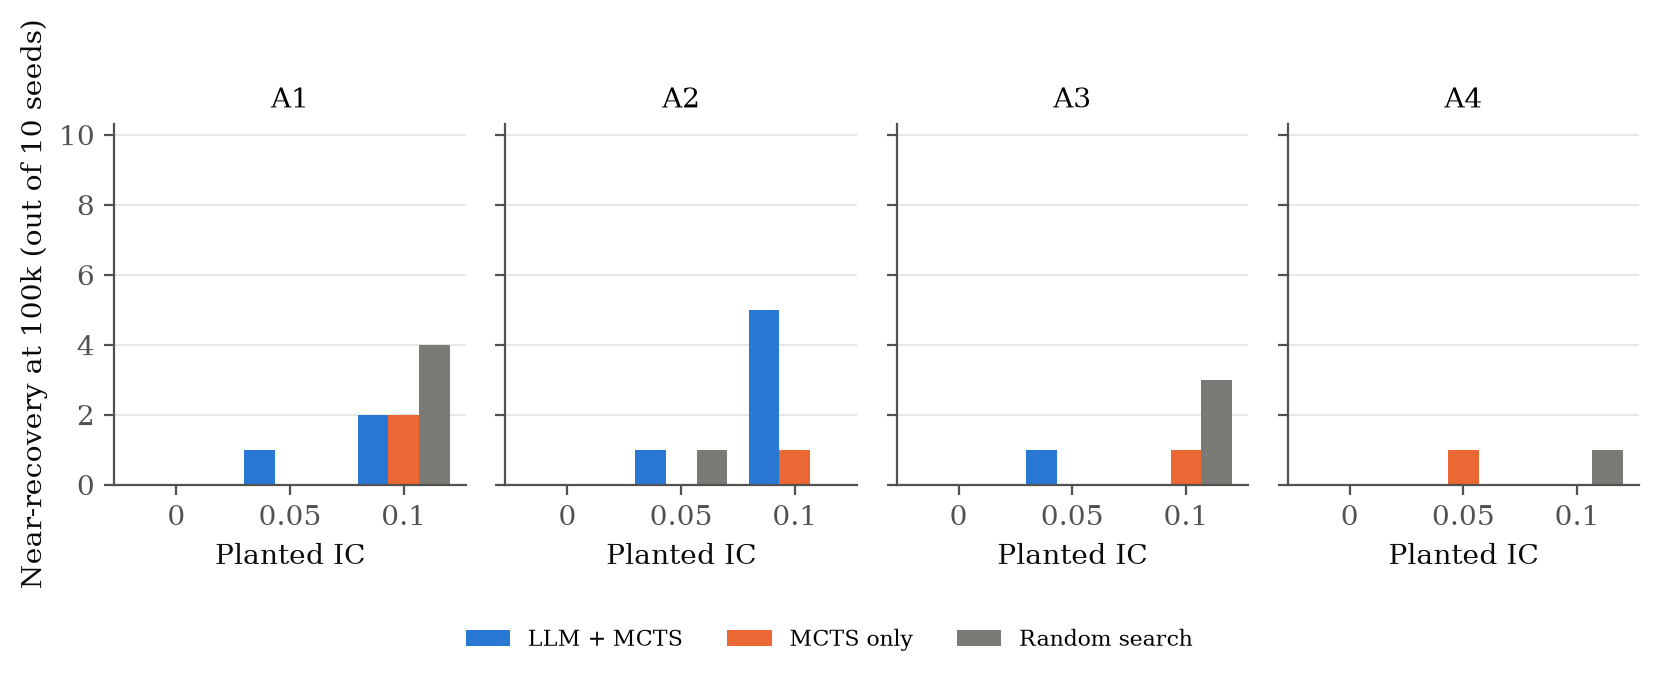
\includegraphics[width=0.95\textwidth]{figures/planted_ic.png}
\caption{Near recoveries at 100,000 evaluations by planted IC}
\label{fig:planted-ic}
\end{figure}

\begin{figure}[H]
\centering
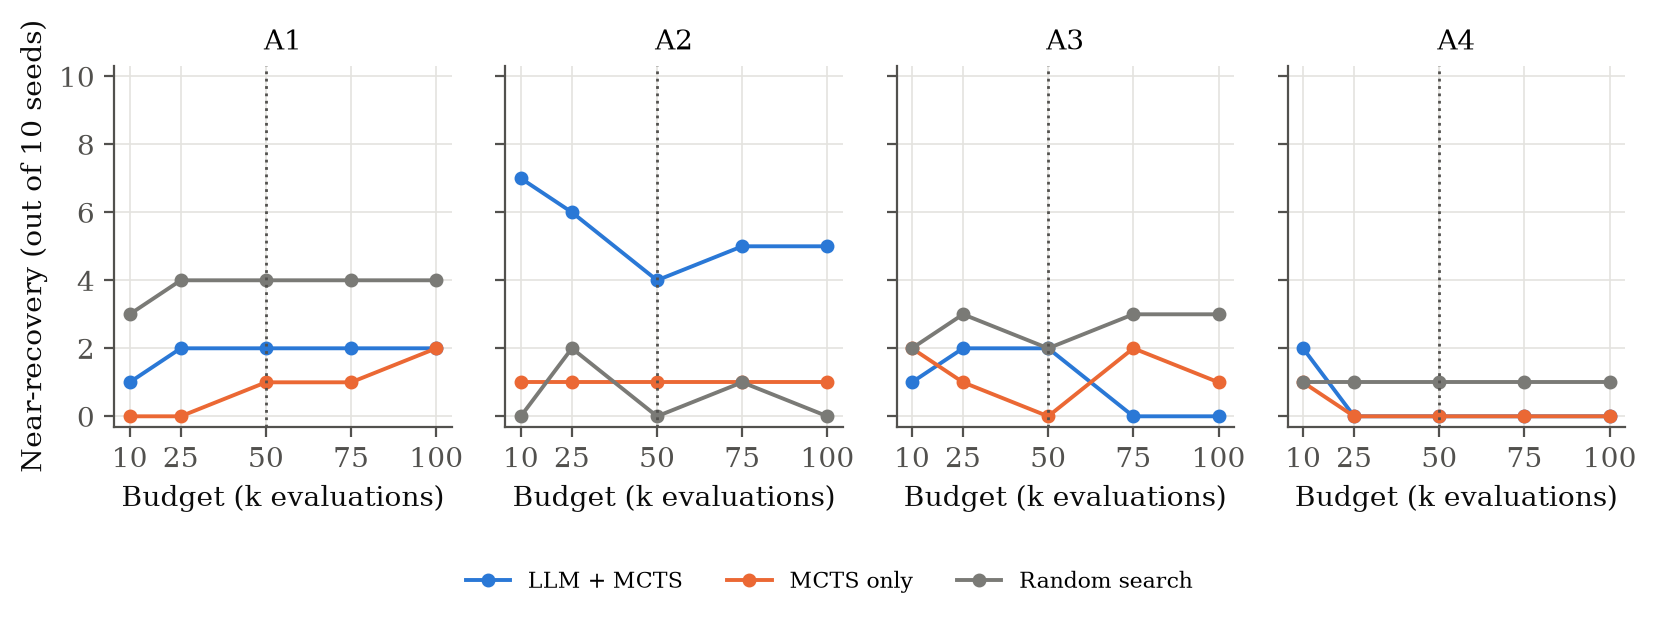
\includegraphics[width=0.95\textwidth]{figures/planted_budget.png}
\caption{Near recoveries at IC 0.1 by budget checkpoint; the dotted line marks the feedback round}
\label{fig:planted-budget}
\end{figure}

The recovery curves are not monotone in the budget (Figure~\ref{fig:planted-budget}): a formula close to $A$ can enter the top five at one checkpoint and leave it at the next, because each checkpoint re-selects the five best of the current leaderboard on validation, and better-scoring formulas found later on the training segment may displace it.

\subsection{Sensitivity to the Recovery Threshold}

The advantage of LLM + MCTS on classical signals comes entirely from A2 and depends on the conventional threshold of 0.7. Table~\ref{tab:threshold} pools A1 and A2 at IC 0.1 and 100,000 evaluations.

\begin{table}[H]
\centering
\caption{Near recoveries of A1 + A2 at IC 0.1, 100,000 evaluations (out of 20), by threshold on $|\rho_S|$}
\label{tab:threshold}
\setstretch{1.1}
\begin{tabular}{lccc}
\toprule
\textbf{Threshold} & \textbf{LLM + MCTS} & \textbf{MCTS only} & \textbf{Random search} \\
\midrule
0.7 & 7 & 3 & 4 \\
0.8 & 3 & 2 & 3 \\
0.9 & 1 & 0 & 3 \\
\bottomrule
\end{tabular}
\end{table}

At 0.9 random search recovers the classical signals most often; the A2 result of LLM + MCTS falls from 5 of 10 at threshold 0.7 to 1 at 0.8 and 0 at 0.9. LLM + MCTS tends to find formulas that resemble A2 rather than A2 itself.

\subsection{RQ2: Detection Threshold}

Only A2 has a detection threshold within the levels run: at IC 0.1, LLM + MCTS recovered it in 5 of 10 runs against 0 of 10 at IC 0 (one-sided Fisher $p = 0.016$). A1, A3 and A4 were not detected at any level. Since one signal passed at IC 0.1, the pre-registered extension to IC 0.2 was not triggered. An IC of 0.1 on 60-minute bars is a strong signal; for comparison, the best formulas reported in cross-sectional studies have ICs of about 0.05 \cite{shi2026}.

\subsection{Reachability of the Planted Signals}

The design planned to read each result according to whether $A$ lies inside the region covered by the initial blueprints. Structurally, only A4 matches a blueprint pattern (\code{ts\_argmax(?)}). However, the blueprint \code{sub(?, ?)} admits $A - c$ for any constant $c$, which trades exactly like $A$ under the NORMALIZED template, so all four signals are reachable from the initial set; one LLM + MCTS run held \code{ts\_argmin(volume, 10) - 2.0}, a copy of A3, in its top five at 10,000 evaluations. The inside/outside reading is therefore not available, and the results are read per signal only.

\subsection{Search Diversity}

The configurations also differ in how broad their leaderboards stay. The median number of distinct expressions among the top 100 fell for MCTS only from 95 at 10,000 evaluations to 30 at 100,000, while LLM + MCTS went from 96 to 86 and random search from 96 to 97. MCTS without the LLM concentrates on a few formulas and their variations; the blueprints keep LLM + MCTS spread over many structures.

\subsection{Health of the Feedback Round}

In the 90 LLM + MCTS runs of the benchmark, the feedback round failed and fell back to the initial blueprints three times (two replies exceeded the context, one produced no acceptable blueprint); 37 runs needed at least one retry because a reply was cut off. Feedback therefore operated as designed in 87 of 90 runs.

\section{Placebo Distribution}
\label{sec:res-placebo}

The 19 placebo runs of LLM + MCTS took 16 hours. Their out-of-sample Sharpe ratios have mean $-0.15$, standard deviation 0.58 and median $-0.38$, range $-0.94$ to 1.04, with 7 of 19 positive (Figure~\ref{fig:placebo}). The mean does not differ from zero ($t \approx -1.15$), and the spread matches the theoretical standard error of a Sharpe ratio over 3.5 years (0.54): the pipeline does not manufacture profits on data without signal, but a single run can still reach a Sharpe ratio near 1 by luck. To obtain $p = 0.05$ the real run had to exceed 1.04; to obtain $p = 0.10$, 0.74.

The feedback round fell back to the initial blueprints in 8 of 133 placebo runs, all because the reply exceeded the context after three attempts. About 10.6\% of evaluations failed on constant-only expressions, as in every configuration.

\section{Real Walk-Forward Run}
\label{sec:res-real}

\subsection{RQ2: Real Run Against Placebo}

The real LLM + MCTS run with seed 1 reached an out-of-sample Sharpe ratio of \textbf{0.68}. Two placebo runs were at least as high (1.04 and 0.74), so $p = 3/20 = 0.15$: the real result is not distinguishable from what the procedure produces on data without predictable structure. The other four seeds reached 0.21, 0.22, 0.47 and 0.26; seed 1 happens to be the best of the five, so the p-value is, if anything, favourable to the real run.

\begin{figure}[H]
\centering
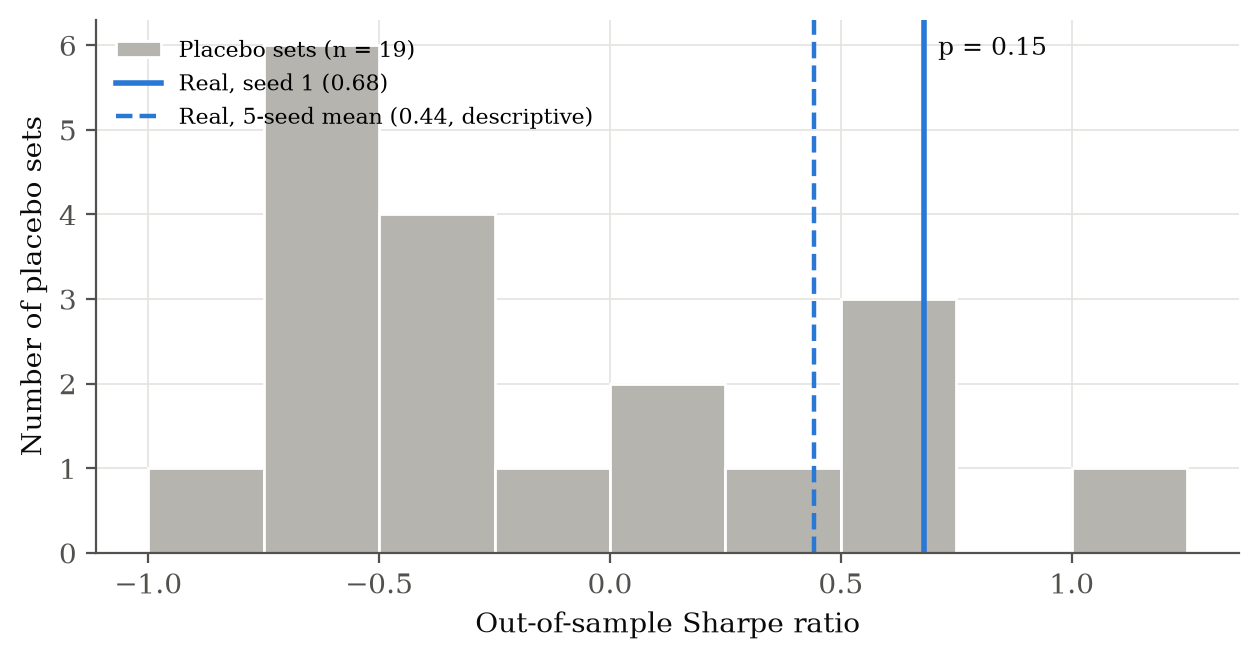
\includegraphics[width=0.85\textwidth]{figures/placebo.png}
\caption{Out-of-sample Sharpe ratios of the 19 placebo runs and of the real run (seed 1); the dashed line is the descriptive five-seed mean}
\label{fig:placebo}
\end{figure}

\subsection{RQ1: Configurations Compared}

Tables~\ref{tab:real-seeds} and \ref{tab:real} report all configurations. LLM + MCTS, MCTS only and random search are almost identical on the five-seed mean series (0.44, 0.40, 0.46), and the seed-to-seed spread within each configuration (for example $-0.40$ to 0.99 for MCTS only) is far larger than the differences between them (Figure~\ref{fig:seeds}). Every 95\% interval of the Sharpe difference contains zero. The search configurations are strongly correlated with each other ($\rho \approx 0.8$), which makes the comparison as sensitive as the data allow, and still no difference appears. The mean series of LLM + MCTS has a higher Sharpe ratio (0.44) than the average of its five seeds (0.37), because averaging five portfolios lowers volatility; this is why the placebo p-value uses a single seed.

\begin{table}[H]
\centering
\caption{Real walk-forward run: annualised out-of-sample Sharpe ratio per seed, 877 days (July 2022 -- December 2025)}
\label{tab:real-seeds}
\setstretch{1.1}
\small
\begin{tabular}{lcccccc}
\toprule
\textbf{Configuration} & \textbf{Seed 1} & \textbf{Seed 2} & \textbf{Seed 3} & \textbf{Seed 4} & \textbf{Seed 5} & \textbf{Mean series} \\
\midrule
LLM + MCTS & 0.68 & 0.21 & 0.22 & 0.47 & 0.26 & 0.44 \\
MCTS only & 0.12 & 0.70 & $-$0.40 & 0.99 & 0.18 & 0.40 \\
Random search & 0.67 & 0.77 & 0.95 & $-$0.67 & $-$0.11 & 0.46 \\
LLM only & 1.10 & & & & & 1.10 \\
Buy-and-hold & 0.67 & & & & & 0.67 \\
TSMOM & 0.08 & & & & & 0.08 \\
\bottomrule
\end{tabular}
\end{table}

\begin{table}[H]
\centering
\caption{Sharpe ratio of LLM + MCTS minus that of each configuration (mean series), paired stationary bootstrap}
\label{tab:real}
\setstretch{1.1}
\small
\begin{tabular}{lcccc}
\toprule
\textbf{Configuration} & \textbf{Difference} & \textbf{95\% CI} & $\bm{\rho}$ & \textbf{Trades per window} \\
\midrule
LLM + MCTS & -- & -- & -- & 509 \\
MCTS only & $+$0.04 & [$-$0.58, 0.67] & 0.81 & 298 \\
Random search & $-$0.02 & [$-$0.64, 0.59] & 0.79 & 444 \\
LLM only & $-$0.66 & [$-$1.59, 0.27] & 0.65 & 519 \\
Buy-and-hold & $-$0.23 & [$-$1.57, 1.03] & 0.07 & 1 \\
TSMOM & $+$0.37 & [$-$1.05, 1.75] & $-$0.07 & 44 \\
\bottomrule
\end{tabular}
\end{table}

\begin{figure}[H]
\centering
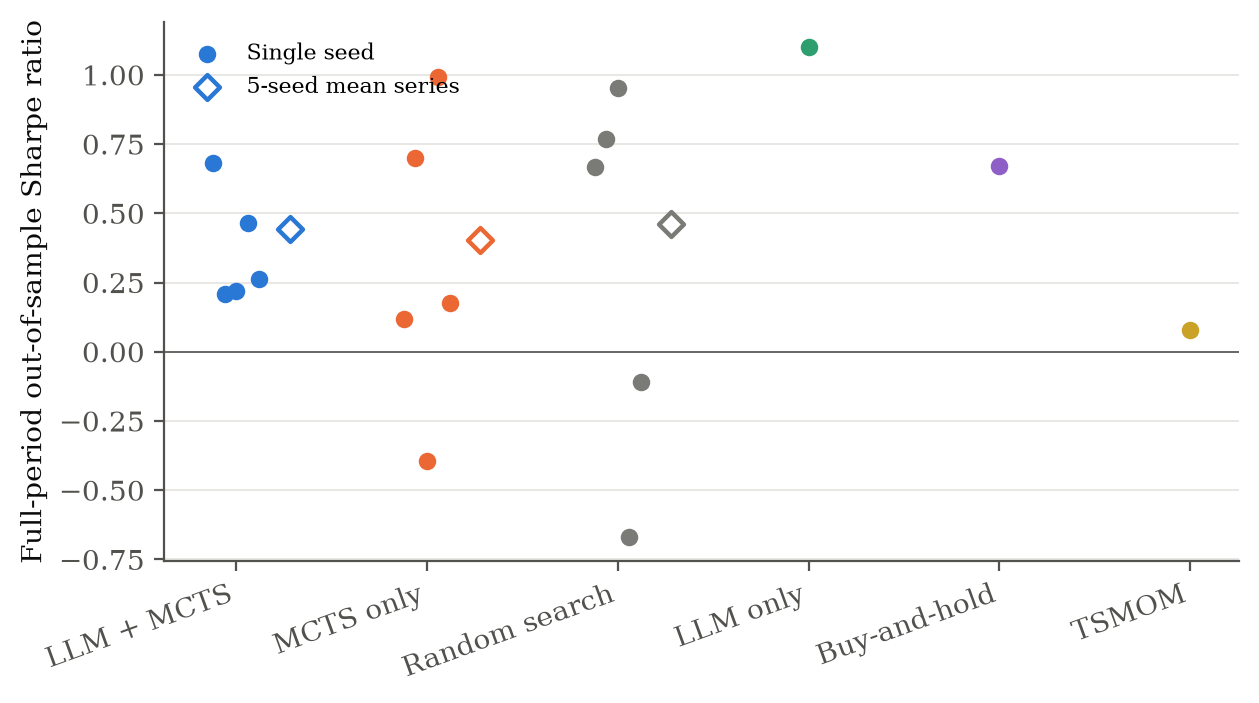
\includegraphics[width=0.85\textwidth]{figures/seed_sharpe.png}
\caption{Out-of-sample Sharpe ratio per seed and of the five-seed mean series}
\label{fig:seeds}
\end{figure}

The LLM-only configuration has the highest Sharpe ratio, 1.10. It is a single selection from one frozen formula set, without placebo runs, and most of its return comes from windows 1 and 7 (window Sharpe ratios 2.41 and 3.98), as Figure~\ref{fig:window} shows. Its difference from LLM + MCTS is not significant either. Buy-and-hold reached 0.67 and TSMOM 0.08.

\begin{figure}[H]
\centering
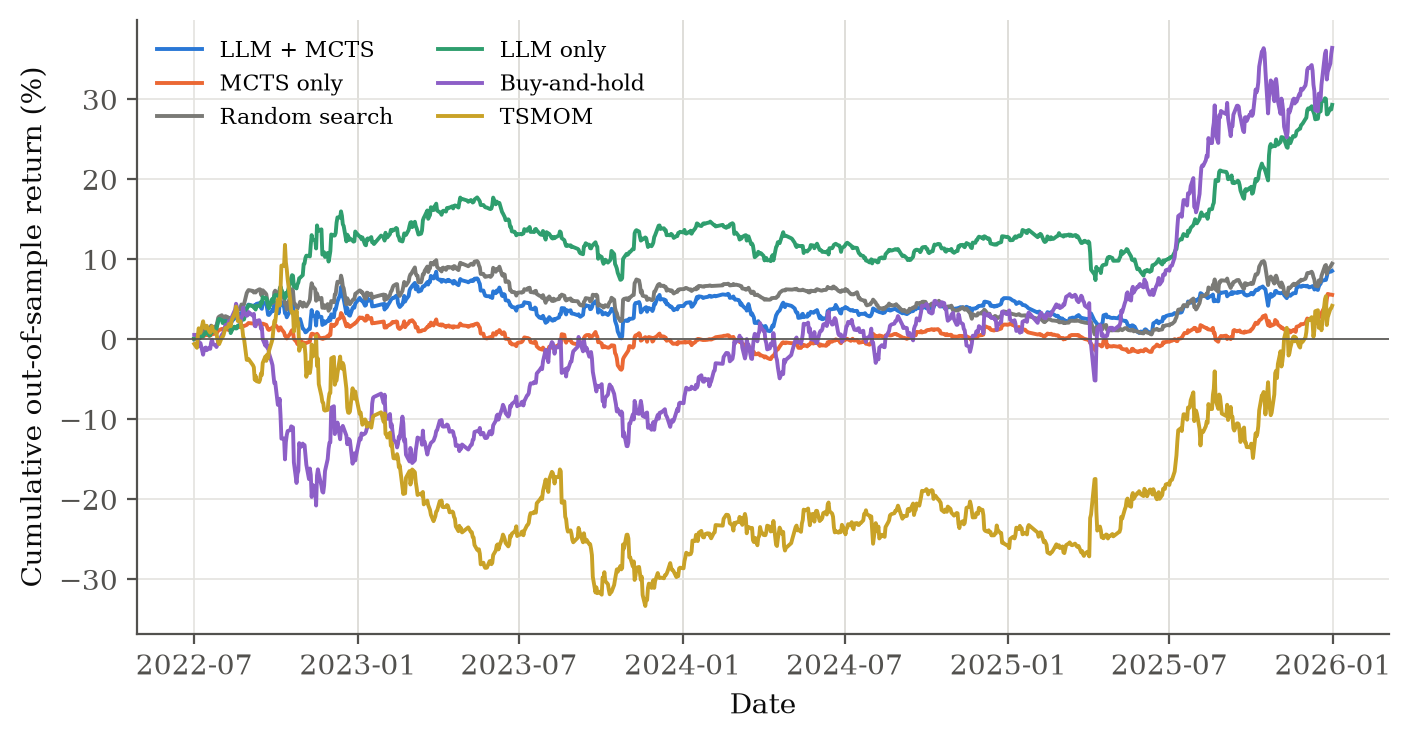
\includegraphics[width=0.95\textwidth]{figures/oos_equity.png}
\caption{Cumulative out-of-sample return of each configuration (mean of five seeds for the search configurations)}
\label{fig:equity}
\end{figure}

\begin{figure}[H]
\centering
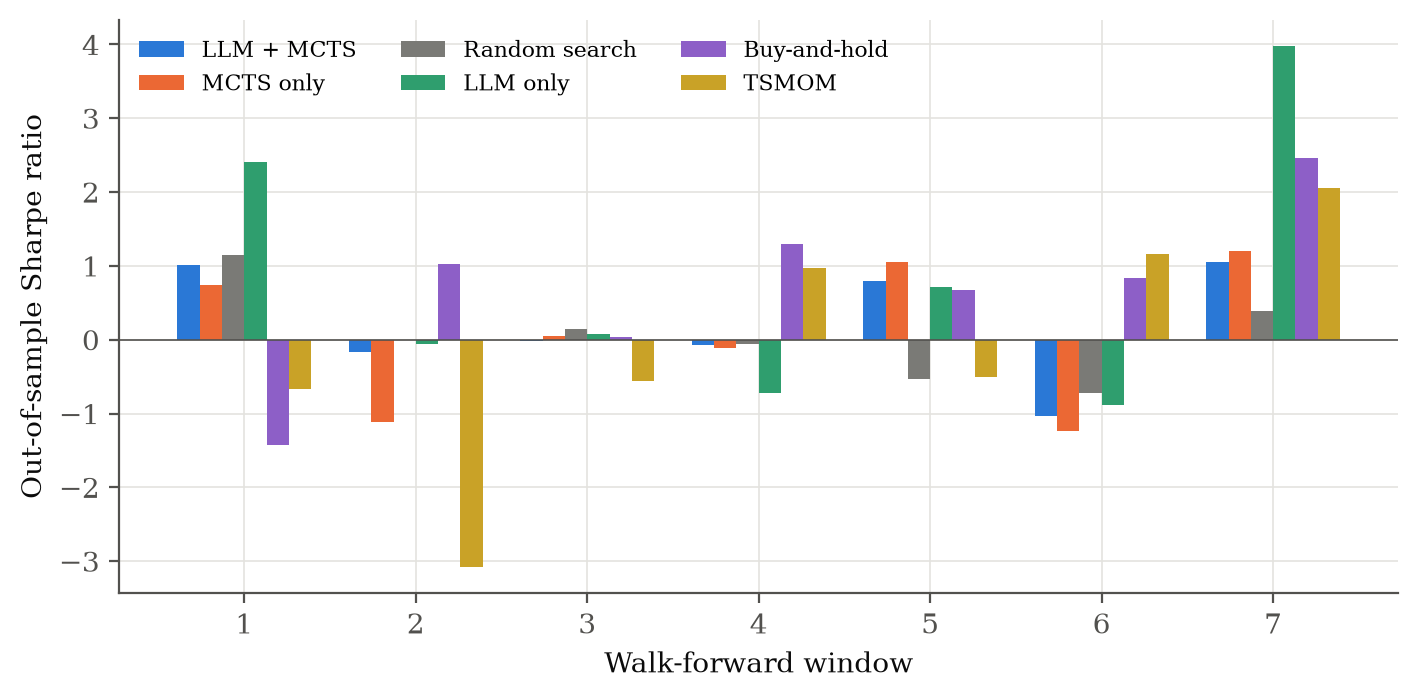
\includegraphics[width=0.95\textwidth]{figures/window_sharpe.png}
\caption{Out-of-sample Sharpe ratio by window (mean over seeds)}
\label{fig:window}
\end{figure}

Window by window (Figure~\ref{fig:window}), the three search configurations were positive in windows 1 and 7 and negative in window 6 (first half of 2025). LLM + MCTS and MCTS only were also positive in window 5, where random search lost, and MCTS only lost in window 2. Buy-and-hold has the opposite profile in several windows: it lost in window 1 (second half of 2022, a falling market) and gained in windows 2, 4 and 7.

\subsection{Feedback Round in the Real Run}

In the 35 real LLM + MCTS runs, the feedback round fell back to the initial blueprints twice (context exceeded) and needed a retry in 17 runs. Evaluation failures on constant-only expressions were 10.6\% for LLM + MCTS and 8.2\% for MCTS only. The real run took 3 hours 37 minutes for LLM + MCTS and 3 hours 46 minutes for the five other configurations together.

\ifdsr
\subsection{Supplementary: Deflated Sharpe Ratio}
\label{sec:dsr}

The Deflated Sharpe Ratio \cite{bailey2014} asks whether a Sharpe ratio exceeds what the best of $N$ trials would reach without skill. Treating each of the 18 real out-of-sample series (five seeds of three search configurations and one series of each deterministic configuration) as a trial, the expected maximum Sharpe ratio under the null, computed from the variance of the 18 daily Sharpe ratios, is 0.89 per year. The Probabilistic Sharpe Ratio of each series against this benchmark, which accounts for the skewness and the fat tails of daily returns (kurtosis 6.8 to 41), gives the DSR. No series reaches the conventional 0.95: the highest are LLM only (0.65, against a PSR of 0.98 relative to zero), MCTS only seed 4 (0.58) and random search seed 3 (0.54); LLM + MCTS seed 1 has 0.35. The 18 trials are not independent (ten series come from two MCTS configurations sharing a grammar, and three configurations contribute one series each), so $N$ and the variance are approximations; the conclusion agrees with the placebo test.
\fi

\section{Leakage Through the LLM's Weights}
\label{sec:leakage}

The model may have read texts about the Vietnamese market in 2020--2025, the period it is evaluated on. Its training cut-off is not published, and the model was released in early 2026. Asked for month-end VN30 levels for 72 months of 2020--2025, it answered almost constants (12 distinct values for 60 months; one value repeated 27 times) and refused or repeated years from April 2025. Its mean relative error (0.197) was worse than guessing the true mean every month (0.183), and its monthly up/down calls were right 48.6\% of the time, below always predicting the majority class (58.3\%). The model therefore carries no usable information about the VN30 price path at a monthly scale. Subtler leakage, such as knowledge of which formulas worked, cannot be excluded, but blueprints were generated with the market name hidden and without any data.

%══════════════════════════════════════════════════════════════════════════════
\chapter{DISCUSSION}
\label{ch5}

\section{Answers to the Research Questions}

\textbf{RQ1 (role of the LLM).} On planted signals, the LLM did not raise the recovery rate of MCTS: none of the four primary tests is significant (Holm-adjusted $p \ge 0.94$). Its only advantage, on A2, depends on the recovery threshold and disappears at 0.8. In the real walk-forward run, LLM + MCTS, MCTS without the LLM and random sampling of the same grammar reach the same out-of-sample performance. Within the power of these experiments, the 4-billion-parameter LLM neither helps nor blocks the search, and MCTS itself does no better than random sampling under the same budget. What the blueprints do change is diversity: they keep the leaderboard spread over many structures where MCTS alone narrows onto a few.

\textbf{RQ2 (evidence of discovery).} The full system's out-of-sample Sharpe ratio of 0.68 is matched or exceeded by 2 of 19 placebo runs ($p = 0.15$). The procedure detects a planted signal of IC 0.1 in one case out of four and none at IC 0.05. There is therefore no evidence that the system discovers more than chance on VN30F1M, and the planted-signal benchmark shows that a negative answer is informative only about signals of roughly IC 0.1 or stronger, of the kind the procedure can detect.

\section{Interpretation}

Three readings of the negative result are possible. The market may contain no edge expressible in the grammar after costs; the procedure may be too weak to find an edge that exists; or the data may be too short to show it. The protocol separates these only partly. The placebo test shows that the selection bias of the procedure is large: the best of 19 runs on permuted data reaches a Sharpe ratio of 1.04, so any real result below that is uninformative regardless of how good it looks. The planted-signal test shows that the procedure is not blind, since it finds A2 at IC 0.1, but also that it is far from reliable: three planted signals of the same strength were missed. And the walk-forward period can confirm only Sharpe ratios above about one. A modest real edge, say a Sharpe ratio of 0.5, would be invisible to all three.

The LLM-only configuration reached the highest Sharpe ratio. Because the LLM never saw data, this cannot be selection on the evaluation period; but the formula set was generated once, there are no placebo runs to calibrate it, its result rests on two windows, and its difference from the other configurations is not significant. It suggests a hypothesis for future work, that simple formulas written from general knowledge are a competitive baseline, rather than a finding.

The results agree with those of Shi et al. \cite{shi2026}, whose direct LLM formulas were no better than random, and contrast with the large gains usually reported for LLM-guided search. The main differences are that this thesis uses a small local model instead of a large cloud model, a single instrument instead of a cross-section, and baselines run under the same budget; the literature reviewed in Chapter~\ref{ch2} did not include a random search or an LLM-free ablation under equal budget, nor a placebo calibration.

\section{Limitations}

\begin{enumerate}
  \item \textbf{One instrument, one frequency.} Results concern VN30F1M at 60-minute bars over 2018--2025 and do not generalise to cross-sectional equities or other frequencies.
  \item \textbf{Statistical power.} 877 out-of-sample days detect only Sharpe differences of about one; ten seeds per planted cell detect only large differences in recovery rates (of the order of 6 of 10 against 1 of 10).
  \item \textbf{One small LLM.} Larger models may behave differently; LLM capability in return prediction grows with model size \cite{lopezlira2023}.
  \item \textbf{Single placebo seed.} Each placebo set was run with one MCTS seed; running five seeds per set would have cost about 64 additional hours.
  \item \textbf{Failed evaluations.} About 7--11\% of evaluations fail on constant-only expressions in every configuration. The rate is similar across configurations, and correcting it would have required rerunning every result.
  \item \textbf{Trade counts.} The real LLM + MCTS run traded far more often (median 509 trades per window) than its placebo runs (48). The difference is not explained; it does not change the p-value, which compares returns after costs, but it suggests that the formulas selected on real data react to features, such as volume patterns, that permutation removes.
  \item \textbf{First-touch timing.} The benchmark recorded when each configuration first touched $A$, in blocks of 500 iterations. Because LLM + MCTS rotates through 20 blueprints, this measure cannot support a claim that one configuration finds $A$ faster, and it is not used.
  \item \textbf{Leakage.} The leakage check covers price levels and directions at a monthly scale only.
\end{enumerate}

%══════════════════════════════════════════════════════════════════════════════
\chapter{CONCLUSION AND FUTURE STUDY}
\label{ch6}

\section{Conclusion}

This thesis evaluated an LLM-guided, dimension-constrained MCTS system for VN30F1M index futures by testing the discovery procedure rather than its output. The configuration was frozen before the real data were used; the procedure was run in seven walk-forward windows, compared with an LLM-free MCTS, random search, the LLM alone and two simple references under the same budget, calibrated against 19 placebo runs of the whole procedure, and checked on four planted signals of known strength.

The answer is negative on both questions. The full system's out-of-sample Sharpe ratio of 0.68 lies within the placebo distribution ($p = 0.15$), and neither the planted-signal benchmark nor the real run shows any advantage of LLM guidance over MCTS alone or over random sampling of the same grammar. The protocol itself is the main contribution: without the placebo runs, a Sharpe ratio of 0.68 after costs, or the 1.10 of the LLM-only configuration, could easily have been reported as a discovery.

\section{Future Study}

\begin{enumerate}
  \item Run the placebo with several MCTS seeds per set and with more sets ($K = 39$ halves the smallest attainable p-value), and add placebo runs for the LLM-only configuration.
  \item Repeat the comparison with larger LLMs and with several feedback rounds, to see whether the null result is specific to a 4-billion-parameter model.
  \item Extend the planted-signal benchmark to more signals of the same IC and to IC 0.2, and measure the time to first recovery with a design that does not rotate blueprints.
  \item Remove constant-only expressions from the grammar before evaluation.
  \item Apply the protocol to other instruments, to finer bar frequencies once the missing sessions are restored, and to cross-sectional universes, where statistical power is much higher.
  \item Compare primitive operators with technical indicators, the question dropped from the proposal.
\end{enumerate}

%══════════════════════════════════════════════════════════════════════════════
\addcontentsline{toc}{chapter}{Bibliography}
\begin{thebibliography}{99}

\bibitem{arian2024}
Arian, H. R., Norouzi Mobarekeh, D., \& Seco, L. A. (2024). Backtest overfitting in the machine learning era: A comparison of out-of-sample testing methods in a synthetic controlled environment. \textit{Knowledge-Based Systems}, 305.

\bibitem{aronson2006}
Aronson, D. (2006). \textit{Evidence-based technical analysis: Applying the scientific method and statistical inference to trading signals}. Wiley.

\bibitem{bailey2014}
Bailey, D. H., \& L\'opez de Prado, M. (2014). The deflated Sharpe ratio: Correcting for selection bias, backtest overfitting and non-normality. \textit{The Journal of Portfolio Management}, 40(5), 94-107.

\bibitem{bailey2017}
Bailey, D. H., Borwein, J. M., L\'opez de Prado, M., \& Zhu, Q. J. (2017). The probability of backtest overfitting. \textit{Journal of Computational Finance}, 20(4), 39-69.

\bibitem{browne2012}
Browne, C. B., Powley, E., Whitehouse, D., Lucas, S. M., Cowling, P. I., Rohlfshagen, P., Tavener, S., Perez, D., Samothrakis, S., \& Colton, S. (2012). A survey of Monte Carlo tree search methods. \textit{IEEE Transactions on Computational Intelligence and AI in Games}, 4(1), 1-43.

\bibitem{glasserman2023}
Glasserman, P., \& Lin, C. (2023). Assessing look-ahead bias in stock return predictions generated by GPT sentiment analysis. \textit{arXiv preprint arXiv:2309.17322}.

\bibitem{hamilton1989}
Hamilton, J. D. (1989). A new approach to the economic analysis of nonstationary time series and the business cycle. \textit{Econometrica}, 57(2), 357-384.

\bibitem{hansen2005}
Hansen, P. R. (2005). A test for superior predictive ability. \textit{Journal of Business \& Economic Statistics}, 23, 365-380.

\bibitem{harvey2015}
Harvey, C. R., \& Liu, Y. (2015). Backtesting. \textit{The Journal of Portfolio Management}, 42(1), 13-28.

\bibitem{harvey2016}
Harvey, C. R., Liu, Y., \& Zhu, H. (2016). \ldots and the cross-section of expected returns. \textit{The Review of Financial Studies}, 29(1), 5-68.

\bibitem{holm1979}
Holm, S. (1979). A simple sequentially rejective multiple test procedure. \textit{Scandinavian Journal of Statistics}, 6(2), 65-70.

\bibitem{kakushadze2016}
Kakushadze, Z. (2016). 101 formulaic alphas. \textit{Wilmott}, 2016(84), 72-80.

\bibitem{kocsis2006}
Kocsis, L., \& Szepesv\'ari, C. (2006). Bandit based Monte-Carlo planning. In \textit{Machine Learning: ECML 2006}, Lecture Notes in Computer Science, vol. 4212 (pp. 282-293). Springer.

\bibitem{koza1992}
Koza, J. R. (1992). \textit{Genetic programming: On the programming of computers by means of natural selection}. MIT Press.

\bibitem{kunsch1989}
K\"unsch, H. R. (1989). The jackknife and the bootstrap for general stationary observations. \textit{The Annals of Statistics}, 17(3), 1217-1241.

\bibitem{ledoit2008}
Ledoit, O., \& Wolf, M. (2008). Robust performance hypothesis testing with the Sharpe ratio. \textit{Journal of Empirical Finance}, 15(5), 850-859.

\bibitem{lo2002}
Lo, A. W. (2002). The statistics of Sharpe ratios. \textit{Financial Analysts Journal}, 58(4), 36-52.

\bibitem{lopezdeprado2018}
L\'opez de Prado, M. (2018). \textit{Advances in financial machine learning}. Wiley.

\bibitem{lopezlira2023}
Lopez-Lira, A., \& Tang, Y. (2023). Can ChatGPT forecast stock price movements? Return predictability and large language models. \textit{arXiv preprint arXiv:2304.07619}.

\bibitem{madaan2023}
Madaan, A., Tandon, N., Gupta, P., Hallinan, S., Gao, L., Wiegreffe, S., Alon, U., Dziri, N., Prabhumoye, S., Yang, Y., Gupta, S., Majumder, B. P., Hermann, K., Welleck, S., Yazdanbakhsh, A., \& Clark, P. (2023). Self-Refine: Iterative refinement with self-feedback. In \textit{Advances in Neural Information Processing Systems 36 (NeurIPS 2023)}.

\bibitem{masters2020}
Masters, T. (2020). \textit{Permutation and randomization tests for trading system development: Algorithms in C++}. Independently published.

\bibitem{moskowitz2012}
Moskowitz, T. J., Ooi, Y. H., \& Pedersen, L. H. (2012). Time series momentum. \textit{Journal of Financial Economics}, 104(2), 228-250.

\bibitem{politis1994}
Politis, D. N., \& Romano, J. P. (1994). The stationary bootstrap. \textit{Journal of the American Statistical Association}, 89(428), 1303-1313.

\bibitem{rabiner1989}
Rabiner, L. R. (1989). A tutorial on hidden Markov models and selected applications in speech recognition. \textit{Proceedings of the IEEE}, 77(2), 257-286.

\bibitem{ren2024}
Ren, T., Zhou, R., Jiang, J., Liang, J., Wang, Q., \& Peng, Y. (2024). RiskMiner: Discovering formulaic alphas via risk seeking Monte Carlo tree search. In \textit{Proceedings of the 5th ACM International Conference on AI in Finance (ICAIF '24)}.

\bibitem{shi2026}
Shi, Y., Duan, Y., \& Li, J. (2026). Navigating the alpha jungle: An LLM-powered MCTS framework for formulaic factor mining. In \textit{Proceedings of the AAAI Conference on Artificial Intelligence}. arXiv:2505.11122.

\bibitem{tang2025}
Tang, Z., Chen, Z., Yang, J., Mai, J., Zheng, Y., Wang, K., Chen, J., \& Lin, L. (2025). AlphaAgent: LLM-driven alpha mining with regularized exploration to counteract alpha decay. \textit{arXiv preprint arXiv:2502.16789}.

\bibitem{wang2023}
Wang, S., Yuan, H., Zhou, L., Ni, L. M., Shum, H.-Y., \& Guo, J. (2023). Alpha-GPT: Human-AI interactive alpha mining for quantitative investment. \textit{arXiv preprint arXiv:2308.00016}.

\bibitem{white2000}
White, H. (2000). A reality check for data snooping. \textit{Econometrica}, 68(5), 1097-1126.

\bibitem{xu2024}
Xu, F., Yin, Y., Zhang, X., Liu, T., Jiang, S., \& Zhang, Z. (2024). Alpha$^2$: Discovering logical formulaic alphas using deep reinforcement learning. \textit{arXiv preprint arXiv:2406.16505}.

\bibitem{yu2023}
Yu, S., Xue, H., Ao, X., Pan, F., He, J., Tu, D., \& He, Q. (2023). Generating synergistic formulaic alpha collections via reinforcement learning. In \textit{Proceedings of the 29th ACM SIGKDD Conference on Knowledge Discovery and Data Mining}.

\end{thebibliography}

\newpage
\appendix

\chapter{Source Code and Reproduction}
\label{app:code}

The source code, the frozen configuration and all result files are available at
\begin{center}
\qrcode[height=3cm]{https://github.com/NguyenTrungAnh-ultra/alpha_farm}\\[2mm]
\url{https://github.com/NguyenTrungAnh-ultra/alpha_farm}
\end{center}
The real walk-forward run used code at commit \code{9d58d63}; its freeze file is \code{results/walkforward/frozen.json}. With Python 3.12 and a local Ollama server serving \code{qwen3.5:4b}, the main results are reproduced by:

\begin{center}
\begin{minipage}{0.92\textwidth}
\small\setstretch{1.1}
\begin{verbatim}
python main.py walkforward placebo --system llm_mcts
python main.py walkforward real --system <configuration>
python main.py walkforward summary --system <configuration>
python main.py rq1 summary
python deflated_sharpe.py
\end{verbatim}
\end{minipage}
\end{center}

\noindent where \code{<configuration>} is one of \code{llm\_mcts}, \code{mcts\_only}, \code{random}, \code{llm\_only}, \code{buy\_hold}, \code{tsmom}, and the real-run commands take the frozen blueprint set \code{results/blueprint\_sets/20261031\_rq1/blueprints.json}. The figures of this thesis are regenerated by \code{docs/thesis/make\_figures.py}.

\chapter{The Frozen Blueprint Set}
\label{app:blueprints}

\begin{table}[H]
\centering
\caption{The 20 initial blueprints (generated by \code{qwen3.5:4b}, seed 2026)}
\label{tab:blueprints}
\setstretch{1.05}
\footnotesize
\begin{tabular}{rll}
\toprule
\# & \textbf{Name (by the LLM)} & \textbf{Blueprint} \\
\midrule
1 & HighVolMeanReversion & \code{not\_(greater\_than(ts\_max(?), ts\_mean(?)))} \\
2 & PriceRangeKinematics & \code{sub(ts\_max(?), ts\_min(?))} \\
3 & ZScoreRegimeDetector & \code{greater\_than(ts\_zscore(?), ts\_rank(?))} \\
4 & OpenCloseSpread & \code{sub(?, ?)} \\
5 & PriceRankSignal & \code{mult(ts\_mean(?), ts\_rank(?))} \\
6 & IndexArgmaxDiff & \code{ts\_argmax(?)} \\
7 & CorrelationArbitrage & \code{not\_(equal(ts\_corr(?), ts\_rank(?)))} \\
8 & ComplexDepthSignal & \code{mult(sub(ts\_max(?), ts\_min(?)), ts\_rank(?))} \\
9 & VolumeWeightedMean & \code{mult(ts\_sum(?), ts\_rank(?))} \\
10 & DeviationCheck & \makecell[l]{\code{or\_(less\_than(ts\_mean(?), ts\_min(?)),}\\\code{\ \ greater\_than(ts\_max(?), ts\_mean(?)))}} \\
11 & MeanReversionHighLow & \code{greater\_than(ts\_max(?), add(ts\_mean(?), ts\_min(?)))} \\
12 & VolatilityWeightedSpread & \code{mult(add(ts\_max(?), ts\_min(?)), ts\_zscore(?))} \\
13 & MeanMinSum & \code{ts\_sum(sub(ts\_mean(?), ts\_min(?)))} \\
14 & PriceChangeKinematics & \code{sub(ts\_sum(?), ts\_mean(?))} \\
15 & VolatilityRegimeMin & \code{ts\_min(sub(ts\_max(?), ts\_mean(?)))} \\
16 & CorrelationMeanScale & \code{mult(ts\_corr(?), ts\_mean(?))} \\
17 & KinematicsAdd & \code{add(ts\_max(?), ts\_min(?))} \\
18 & StatisticalMeanReversion & \code{ts\_mean(add(?, ?))} \\
19 & ZScoreLogic & \code{greater\_than(ts\_sum(?), ts\_max(?))} \\
20 & VolumeCorrelationRank & \code{mult(add(ts\_max(?), ts\_min(?)), ts\_rank(?))} \\
\bottomrule
\end{tabular}
\end{table}

The names are the LLM's own and do not always describe the formula.

\chapter{Development History}
\label{app:history}

Before the feedback round was added, the system generated its blueprints once and ran 20 blueprints $\times$ 5,000 iterations per window. This earlier system was run only on placebo and planted data, never on the real out-of-sample period. Its 19 placebo runs had Sharpe ratios with mean 0.11 and maximum 1.02, close to those of the final system. Its planted-signal benchmark, on a formula derived from its own blueprint set and the segments of walk-forward window 1, gave a detection threshold of IC 0.1 (6 of 10 near recoveries against 0 of 10 at IC 0, $p = 0.005$), and IC 0.05 was not separated from noise (2 of 10, $p = 0.24$). The formula it recovered lay in a blueprint with only 256 completions, so that benchmark measured the ability to rank the right formula into the top five more than the ability to find it; this motivated the four pre-registered signals of the final benchmark.

A first-generation version, searching over technical indicators, produced 171 candidate strategies filtered by robustness tests on HMM-simulated paths \cite{hamilton1989,rabiner1989,kunsch1989}; one survived, and in-sample Sharpe ratios correlated only 0.19--0.24 with performance on simulated paths. These observations, reported in the proposal, motivated the protocol of this thesis. The HMM tests are kept in the code to describe risk only and play no role in the results.

\end{document}
